\documentclass{article}

\usepackage{tikz}
\usepackage{minted}
\usepackage{ifthen}
\usepackage{caption}
\usepackage{subfig}
\usepackage{listings}
\usepackage{geometry}
 \geometry{
	 a4paper,
	 left=25mm,
	 right=20mm,
	 top=20mm,
	 bottom=20mm,
 }

\usetikzlibrary{calc,positioning,shadows.blur,decorations.pathreplacing,decorations.pathmorphing}
\usepackage{etoolbox}


\definecolor{r0d}{RGB}{255,214,226}
\definecolor{r1d}{RGB}{165,201,239}
\definecolor{r2d}{RGB}{196,228,239}

\tikzset{%
	snake it/.style = {decorate, decoration=snake},
  brace/.style = { decorate, decoration={brace, amplitude=5pt} },
  mbrace/.style = { decorate, decoration={brace, amplitude=5pt, mirror} },
  label/.style = { black, midway, scale=0.8, align=center },
  toplabel/.style = { label, above=.5em, anchor=south },
  leftlabel/.style = { label,rotate=90,left=1.9em,anchor=north },   
  rightlabel/.style = { label,rotate=-90,right=1.5em,anchor=north },   
  bottomlabel/.style = { label, below=.5em, anchor=north },
  force/.style = { rotate=-90,scale=0.4 },
  round/.style = { rounded corners=2mm },
  legend/.style = { right,scale=0.4 },
  nosep/.style = { inner sep=0pt },
  generation/.style = { anchor=base }
}


\begin{document}

\title{Block Sparse Matrix-Vector Multiplication with CUDA}
\author{Georgii Evtushenko}

\maketitle

In the previous post, we've discussed sparse matrix-vector multiplication. It was shown that it's possible to take advantage 
of knowledge about a position of zeroes by storing matrices in special data structures. Although we've improved performance 
and memory space requirements, we haven't used all the information about zeroes position. In some applications, non-zeroes 
are gathered in blocks. The knowledge about these blocks could give us more room for optimization. In this post, I'm going 
to discuss the efficiency of block sparse matrix-vector multiplication on GPU. To show some real-live application results, 
I develop a Matrix Structural Analysis application, which is used to simulate the Golden Gate bridge structure. 

\section{Block Compressed Sparse Row (BCSR)}
BCSR is one of the most popular block sparse matrix formats. In BCSR, all blocks have the same size. To understand this 
format imagine a sparse matrix with the block size equal to one. In this case, CSR and BCSR matrix representations are 
equivalent. Block size increasing doesn't affect the column and row pointer arrays. Instead, it just extends the values 
array. That is, columns and row pointer arrays contain values for blocks. Blocks are stored in the value array contiguously. 

\begin{figure}[H]
  \centering
  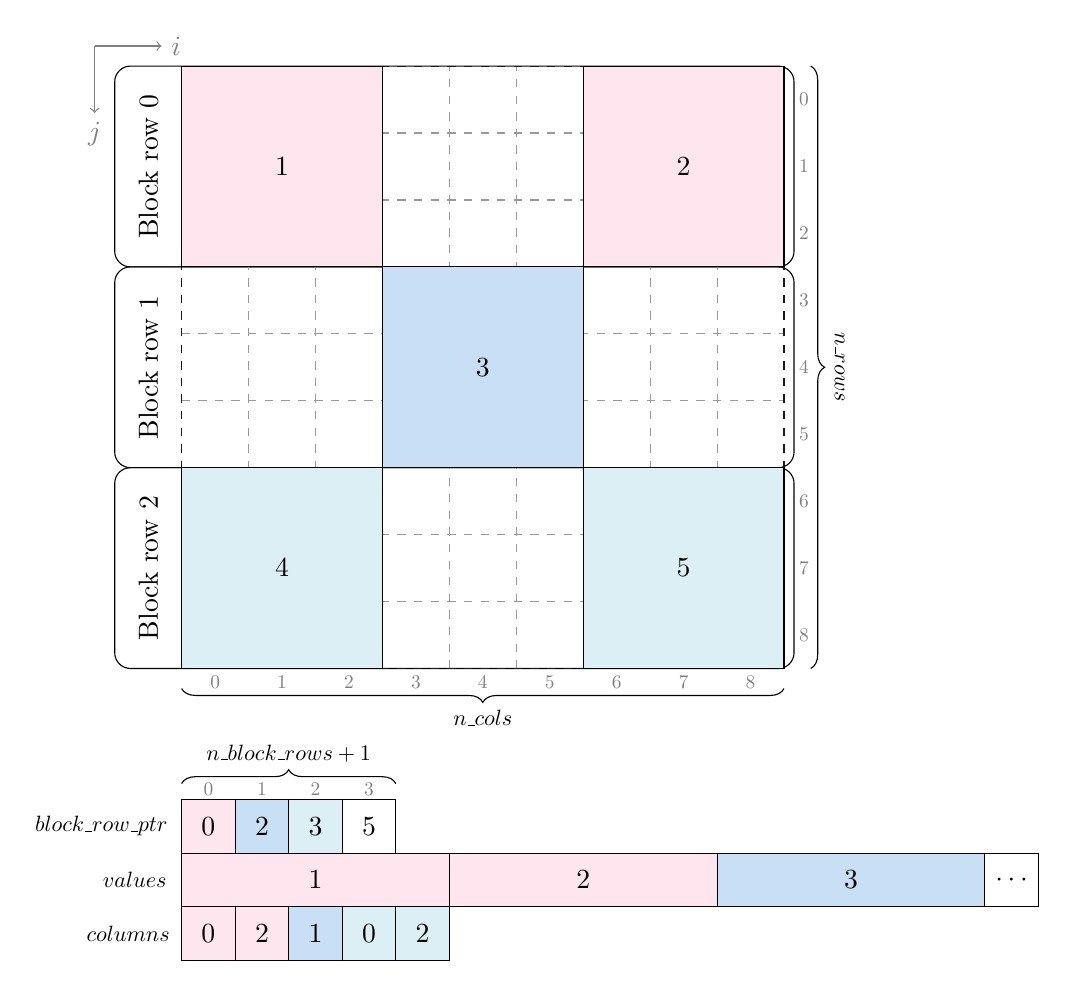
\begin{tikzpicture}[circ/.style = {circle, draw, inner sep=0pt, minimum size=3pt, outer sep=0pt, minimum size=6mm}, scale=0.85]

  \draw[round] (-1.0,6.0) rectangle (9.15,9);
  \draw[round] (-1.0,3.0) rectangle (9.15,6);
  \draw[round] (-1.0,0.0) rectangle (9.15,3);
	
  \node[rotate=90] at (-0.5,7.5)   {Block row 0};
  \node[rotate=90] at (-0.5,4.5)   {Block row 1};
  \node[rotate=90] at (-0.5,1.5)   {Block row 2};

  \foreach \y in {0,...,8} {
    \node[scale=0.7,text=gray] at (9.3,9.0 - 1.0*\y - 0.5) {\y};
  }

  \foreach \x in {0,...,8} {
    \node[scale=0.7,text=gray] at (1.0*\x + 0.5,-0.2) {\x};
  }

  \draw[->,gray] (-1.3,9.3) -- (-0.3,9.3) node[right] {$i$};
  \draw[->,gray] (-1.3,9.3) -- (-1.3,8.3) node[below] {$j$};

  % Elements mesh
  \draw[step=1.0,gray!80!white,thin,dashed,line width=0.4] (0.0,0.0) grid (9.0,9.0);
  \draw[step=3.0,black!90!white,thin,dashed,line width=0.4] (0.0,0.0) grid (9.0,9.0);

  % \draw[round] (-0.15,0) rectangle (10.15,10);

  % Right braces
  \draw [mbrace] (9.4,0.0)  -- (9.4,9.0) node[rightlabel] {$n\_rows$};

  % Bottom braces
  \draw [mbrace] (0.0,-0.3) -- (9,-0.3) node[bottomlabel] {$n\_cols$};

  \edef\esize{1.0}

  % ROW 0
  \edef\elementnum{1}
  \foreach \col in {0,2} {
    \draw[fill=r0d!60] (\col*3*\esize,6.0) rectangle (\col*3*\esize+3*\esize,9) node[pos=.5] {\elementnum};
    \pgfmathparse{int(\elementnum+1)}
    \xdef\elementnum{\pgfmathresult}
  }

  % ROW 1
  \foreach \col in {1} {
    \draw[fill=r1d!60] (\col*3*\esize,3.0) rectangle (\col*3*\esize+3*\esize,6) node[pos=.5] {\elementnum};
    \pgfmathparse{int(\elementnum+1)}
    \xdef\elementnum{\pgfmathresult}
  }

  % ROW 1
  \foreach \col in {0,2} {
    \draw[fill=r2d!60] (\col*3*\esize,0.0) rectangle (\col*3*\esize+3*\esize,3) node[pos=.5] {\elementnum};
    \pgfmathparse{int(\elementnum+1)}
    \xdef\elementnum{\pgfmathresult}
  }

  % RHS
  \edef\lasty{0}
  \edef\ynum{1}

  % =====================================================
  % ================== Data structures ================== 
  % =====================================================

  % RHS OFFSETS
  \edef\ybot{-1.0}
  \edef\esize{0.8}

  \edef\xnum{0}
  \edef\lastblockoffset{0}
  \edef\lastyoffset{\ybot-\esize*0.8}

  % ROWS NON ZEROS
  \pgfmathparse{\ybot-\esize*2.2}
  \xdef\ybot{\pgfmathresult}

  % MATRIX OFFSETS
  \draw [mbrace] (4 *\esize,\ybot+1.3*\esize)  -- (0*\esize,\ybot+1.3*\esize) node[toplabel] {$n\_block\_rows+1$};

  \node[scale=0.8] at (-1.2,\ybot+\esize/2) {$block\_row\_ptr$};

  \foreach \i in {0,...,3} {
    \node[scale=0.7,text=gray] at (\i * \esize + \esize/2,\ybot+\esize*1.2) {\i};
  }

  \edef\xnum{0}
  \edef\lastblockoffset{0}
  \edef\middlepoint{\ybot-\esize/2}

  \foreach \offset in {0,2,3,5} {
    \pgfmathparse{\esize*\offset}
    \xdef\lastblockoffset{\pgfmathresult}

    \ifthenelse{\xnum<1}
    { \draw[fill=r0d!60] (\xnum*\esize,\ybot) rectangle (\xnum*\esize+\esize,\ybot+\esize) node[pos=.5] {\offset}; }
    {
      \ifthenelse{\xnum<2}
      { \draw[fill=r1d!60] (\xnum*\esize,\ybot) rectangle (\xnum*\esize+\esize,\ybot+\esize) node[pos=.5] {\offset}; }
      {
        \ifthenelse{\xnum<3}
        { \draw[fill=r2d!60] (\xnum*\esize,\ybot) rectangle (\xnum*\esize+\esize,\ybot+\esize) node[pos=.5] {\offset}; }
        {
          \ifthenelse{\xnum<11}
          { \draw[fill=white] (\xnum*\esize,\ybot) rectangle (\xnum*\esize+\esize,\ybot+\esize) node[pos=.5] {\offset}; }
          { 
          }
        }
      }
    }
    \pgfmathparse{int(\xnum+1)}
    \xdef\xnum{\pgfmathresult}
  }

  % MATRIX DATA
  \pgfmathparse{\ybot-\esize}
  \xdef\ybot{\pgfmathresult}

  \node[scale=0.8] at (-0.7,\ybot+\esize/2) {$values$};

  % Row 0
  \edef\elementnum{1}
  \foreach \i in {0,...,1} {
    \draw[fill=r0d!60]  (\i * 5*\esize,\ybot) rectangle (\i * 5*\esize + 5*\esize,\ybot+\esize) node[pos=0.5] {\elementnum};
    \pgfmathparse{int(\elementnum+1)}
    \xdef\elementnum{\pgfmathresult}
  }
  \foreach \i in {2} {
    \draw[fill=r1d!60]  (\i * 5*\esize,\ybot) rectangle (\i * 5*\esize + 5*\esize,\ybot+\esize) node[pos=0.5] {\elementnum};
    \pgfmathparse{int(\elementnum+1)}
    \xdef\elementnum{\pgfmathresult}
  }

  \draw[fill=white]  (3 * 5*\esize,\ybot) rectangle (3 * 5*\esize + 1*\esize,\ybot+\esize) node[pos=0.5] {$\cdots$};

  \pgfmathparse{\ybot-\esize}
  \xdef\ybot{\pgfmathresult}
  \node[scale=0.8] at (-0.8,\ybot+\esize/2) {$columns$};

  \edef\elementnum{0}
  \foreach \i in {0,2} {
    \draw[fill=r0d!60] (\elementnum * \esize,\ybot) rectangle (\elementnum * \esize + \esize,\ybot+\esize) node[pos=0.5] {\i};
    \pgfmathparse{int(\elementnum+1)}
    \xdef\elementnum{\pgfmathresult}
  }
  \foreach \i in {1} {
    \draw[fill=r1d!60] (\elementnum * \esize,\ybot) rectangle (\elementnum * \esize + \esize,\ybot+\esize) node[pos=0.5] {\i};
    \pgfmathparse{int(\elementnum+1)}
    \xdef\elementnum{\pgfmathresult}
  }
  \foreach \i in {0,2} {
    \draw[fill=r2d!60] (\elementnum * \esize,\ybot) rectangle (\elementnum * \esize + \esize,\ybot+\esize) node[pos=0.5] {\i};
    \pgfmathparse{int(\elementnum+1)}
    \xdef\elementnum{\pgfmathresult}
  }

  \end{tikzpicture}
  \caption{Example of Block Compressed Sparse Row (BCSR) matrix format}
  \label{csr_format}
\end{figure}

To access block rows data, we need to get a number of blocks before the row ($row\_ptr[block\_row]$) and multiply this value
by block size square. It's possible to store blocks in row-major or column-major order. As I'll show further, elements order 
within blocks might affect performance. I'll start with row-major order.

\end{document}
